\documentclass[11pt,a4paper]{article}
\usepackage[utf8]{inputenc}
\usepackage[spanish]{babel}
\usepackage{amsmath}
\usepackage{amsfonts}
\usepackage{amssymb}
\usepackage{graphicx}
\author{Manuel González González}
\title{Práctica 10: Mapa de Kohonen}
\begin{document}
\maketitle

\section*{Ejercicio 1}
\subsection*{a)}
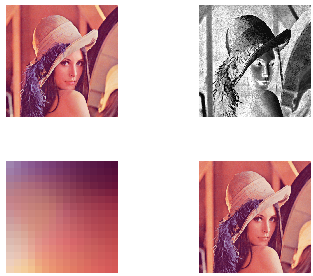
\includegraphics[scale=1]{lena.png}

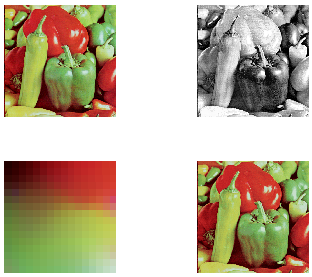
\includegraphics[scale=1]{peppers.png}

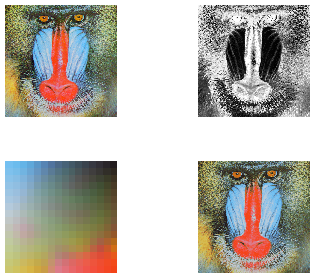
\includegraphics[scale=1]{baboon.png}

\subsection*{b)}

Necesitamos los índices de las neuronas para acceder a las posiciones donde se guardan sus valores.

\subsection*{c)}
Porque en lugar de tener que guardar un mapa de valores con la información de cada píxel, solo nos hace falta guardar la información de los índices de las neuronas entrenadas.

\section*{2}
\subsection*{a)}
En el caso de Lena se obtiene: 13.0676, 15.0288, 15.9873.\\

En el caso de Baboon obtenemos: 46.3253, 56.959, 44.36645.\\

Y por último, para Peppers el vector es: 22.4698, 33.5252, 51.8747.

\subsection*{b)}
La de mayor módulo es Baboon, con 85.7832.

\subsection*{c)}
Por la dispersión de los colores que tiene, lo cual hace que sea más difícil de entrenar la red.

\subsection*{d)}
El tercer componente (Blue) es el que cuenta con mayor error. Esto se debe a que los colores predominantes en la imagen son el verde y el rojo. Por ende, son los que se pueden entrenar mejor.

\end{document}